% AAAI-27 submission — anonymous review version.
% Requires the official AAAI-27 author kit (aaai2027.sty, aaai2027.bst) from
% https://aaai.org/authorkit27/ — see README_BUILD.md for setup and fallback.
\documentclass[letterpaper]{article}
\usepackage[submission]{aaai2027}     % from the AAAI-27 author kit
\usepackage{times}
\usepackage{helvet}
\usepackage{courier}
\usepackage[hyphens]{url}
\usepackage{graphicx}
\usepackage{booktabs}
\usepackage{amsmath}
\urlstyle{rm}
\def\UrlFont{\rm}
\pagestyle{plain}
\pagenumbering{arabic}
\frenchspacing
\setlength{\pdfpagewidth}{8.5in}
\setlength{\pdfpageheight}{11in}

\title{Positional Encoding as a Hidden Variable in Grokking:\\
PE Choice Shifts Grokking Onset and the Attention-Dependence\\
of the Learned Circuit}
\author{Anonymous submission}

\begin{document}
\maketitle

\begin{abstract}
Grokking studies on modular arithmetic conventionally fix the positional-encoding
(PE) scheme, while mechanistic studies of the resulting ``clock/pizza'' circuits
vary attention type---leaving PE an uncontrolled variable in both literatures. We
make PE the controlled independent variable: 50 pre-registered training runs of a
1-layer transformer on $(a+b) \bmod 113$ crossing five PE conditions
\{NoPE, learned, sinusoidal, RoPE, ALiBi\} with matched seeds, data splits, and
optimization. PE modulates \emph{dynamics}: at the standard 15k-epoch horizon,
sinusoidal APE grokked in 0 of 6 runs versus 14 of 24 for all other PEs combined
(Fisher exact $p{=}0.014$, exploratory); 40k-epoch extensions show sinusoidal is
delayed, not blocked (median onset 20{,}980 epochs vs.\ 14{,}350--15{,}215;
every resolved sinusoidal onset exceeds 15{,}650, above 15 of the 20 other-PE
onsets), though omnibus rank tests across all five PEs remain null at five seeds.
At the algorithmic level all grokked runs converge to the same
Fourier-multiplication circuit family (restricted loss $\approx 0$; embedding
Fourier concentration $0.83$--$0.88$)---yet the pre-registered label-permutation
test on six-metric circuit signatures at matched post-grok checkpoints is
strongly positive ($\eta^2{=}0.37$, $p{=}0.001$, $n{=}20$ balanced): PEs acting
on attention (RoPE, ALiBi) yield circuits nearly indifferent to attention
ablation (uniform-attention $\Delta$loss 1.2--2.0), while embedding-level or
absent PEs (learned, sinusoidal, NoPE) yield strongly attention-dependent
circuits ($\Delta$ 4.0--5.6). Finally, a run's circuit signature---not its PE
label---predicts out-of-distribution accuracy on held-out operand ranges
(leave-one-out $R^2$ $0.92$ vs.\ $-1.59$; Spearman $\rho{=}0.94$, $n{=}10$).
PE choice thus leaves the learned algorithm invariant while controlling when it
forms and where it lives---in attention or around it. All experiments are
CPU-scale, deterministic, and fully reproducible from released code, seeds, and
per-epoch logs.
\end{abstract}

\section{Introduction}

Small transformers trained on modular arithmetic exhibit
\emph{grokking}---delayed generalization long after memorization
\cite{power2022grokking}---and have become a model system for mechanistic
interpretability: the generalizing solution is a Fourier-based
multiplication circuit that can be read out of the weights
\cite{nanda2023progress}. A parallel line of work asks \emph{which} internal
algorithm forms, contrasting ``clock'' and ``pizza'' circuits under varied
attention mechanisms \cite{zhong2023clock} and, more recently, arguing these are
parameterizations of one abstract algorithm \cite{mccracken2025universal,
moisescu2025unifying}.

Both literatures treat positional encoding as a fixed implementation detail:
grokking studies conventionally use a learned absolute PE; circuit-multiplicity
studies vary attention, width, or depth. Yet PE directly parameterizes the very
subspace in which these circuits form---the token embedding and the
query--key interaction---and the PE literature itself shows that PE choice has
large effects on what transformers learn to compute
\cite{kazemnejad2023impact}. Whether PE shapes grokking dynamics or the identity
of the learned circuit has, to our knowledge, not been tested.

We pre-registered and ran that test. Holding task, architecture, optimizer, data
fraction, and seeds fixed, we cross five PE conditions---NoPE (no positional
information beyond the causal mask), learned APE, sinusoidal APE
\cite{vaswani2017attention}, RoPE \cite{su2021roformer}, and ALiBi
\cite{press2021train}---and measure (H1) grokking onset and sharpness, (H2)
continuous \emph{circuit signatures} (embedding/logit Fourier concentration,
restricted/excluded loss, attention entropy, uniform-attention ablation), and
(H3) out-of-distribution behavior on held-out operand ranges.

\paragraph{Contributions.}
\begin{itemize}
\item \textbf{PE controls grokking dynamics.} Sinusoidal APE delays grokking
(0/6 runs grokked at the standard 15k-epoch horizon vs.\ 14/24 for other PEs;
all runs grok by 40k; median onset 21.0k vs.\ 14.4--15.2k). Onset differences
among the remaining PEs are within seed noise at $n{=}5$; we report the
pre-registered omnibus nulls in full.
\item \textbf{PE selects the circuit's attention-dependence, not its
algorithm.} All grokked runs converge to the same Fourier circuit family
(extending circuit-universality
\cite{mccracken2025universal,moisescu2025unifying} across the PE axis), yet
post-grok signatures separate strongly by PE ($\eta^2{=}0.37$, $p{=}0.001$):
attention-level PEs (RoPE, ALiBi) produce circuits robust to attention
ablation; embedding-level or absent PEs do not.
\item \textbf{Signatures, not PE labels, predict OOD.} Leave-one-out prediction
of held-out-operand accuracy from circuit signatures achieves $R^2{=}0.92$;
the PE label alone is uninformative ($R^2{=}-1.59$).
\item \textbf{A fully deterministic, CPU-scale, pre-registered experimental
protocol} (50 runs, $\sim$0.23M-parameter models) with per-epoch logs,
log-spaced checkpoints, and single-command reproduction of every figure and
statistic.
\end{itemize}

\section{Related Work}

\paragraph{Grokking.} Delayed generalization on algorithmic tasks was identified
by \citet{power2022grokking}; \citet{nanda2023progress} exhibited the Fourier
circuit and progress measures (restricted/excluded loss) that we adopt.
Weight decay's causal role in the memorization-to-generalization transition has
been mapped as a control parameter \cite{verma2026weight}; we hold it fixed
(1.0) and vary PE instead. \citet{truong2026atgrok} caution that at-grok
checkpoints are not converged; our circuit comparisons therefore use final,
post-early-stop checkpoints.

\paragraph{Circuit identity on modular addition.} \citet{zhong2023clock}
demonstrated multiple algorithmic solutions (clock vs.\ pizza) controlled by
attention type; \citet{furuta2024towards} extended circuit analysis across
modular polynomials. Recent work argues the apparent multiplicity collapses to
one abstract algorithm \cite{mccracken2025universal,moisescu2025unifying}. Our
design differs on the controlled variable: we vary PE, not attention, and find
convergence \emph{across PEs}---evidence for universality along an axis these
studies did not manipulate.

\paragraph{Positional encoding.} PE schemes differ in inductive bias and
length generalization \cite{kazemnejad2023impact}, with NoPE provably able to
recover position from the causal mask. Sinusoidal \cite{vaswani2017attention},
rotary \cite{su2021roformer}, and linear-bias \cite{press2021train} encodings
are standard; to our knowledge no prior work measures their effect on grokking
dynamics or on circuit formation.

\section{Experimental Setup}

\paragraph{Task and data.} Sequences $[a, b, {=}]$ with target
$c=(a{+}b) \bmod p$, $p{=}113$; vocabulary of $p{+}1$ tokens; loss and accuracy
read at the ${=}$ position. Train split: 30\% of all $p^2$ pairs by seeded
permutation; the split seed equals the model seed, and all five PE conditions
share the split within a seed (paired design). Full-batch training; one epoch =
one optimizer step.

\paragraph{Model.} 1-layer decoder-only transformer, $d_{\text{model}}{=}128$,
4 heads, $d_{\text{mlp}}{=}512$, ReLU, no LayerNorm, untied embed/unembed, no
attention biases ($\approx$0.23M parameters)---the configuration of
\citet{nanda2023progress}, chosen for circuit legibility.

\paragraph{PE conditions.} \{NoPE; learned APE; sinusoidal APE; RoPE on
$Q,K$; ALiBi head-specific linear biases\}. Formula-based PEs add no
parameters; learned APE adds $3\times128$.

\paragraph{Optimization.} AdamW, lr $10^{-3}$, weight decay $1.0$, betas
$(0.9, 0.98)$, up to 15{,}000 epochs (extension runs: 40{,}000), early stop
after validation accuracy $\ge 0.99$ sustained for 1{,}000 consecutive epochs.
Onset := first epoch of the sustained window; runs without one are censored.

\paragraph{Runs.} Pre-registered grid: core 5 PE $\times$ 5 seeds; OOD set
5 PE $\times$ 2 seeds with operand rows $a \in [100,112]$ held out of train
and validation; 40k-epoch extensions of all 15 runs censored at the 15k cap
(deterministic seed replay; identical trajectory through the original
horizon). 50 runs total, zero failures; every run is reported.

\paragraph{Circuit signatures.} Six continuous metrics per checkpoint:
embedding Fourier concentration (top-5 non-DC frequency power share); logit
Fourier concentration; \emph{logit-level} restricted and excluded loss
(Fourier projection of the $(a{+}b)$-grouped logit matrix onto its top-5
frequencies---an architecture-agnostic variant of \citet{nanda2023progress}'s
measures, applicable identically under every PE); mean attention entropy at
${=}$; and uniform-attention ablation $\Delta$loss (the discriminator of
\citet{zhong2023clock}). Following the at-grok caution
\cite{truong2026atgrok}, endpoint comparisons use final checkpoints.

\paragraph{Statistics.} Onsets: per-PE medians with bootstrap CIs;
Kruskal--Wallis and pairwise Mann--Whitney (Holm-corrected) on uncensored
onsets; $k$-group log-rank including censored runs. Signatures: permutation
test (10k label shuffles) on the between/total-variance ratio $\eta^2$ of
standardized six-metric vectors. OOD: leave-one-out ridge prediction from
signatures vs.\ PE-label group means. Exploratory analyses are labeled as such.

\section{H1: PE Shifts Grokking Dynamics}

All 25 core-condition runs follow the canonical grokking trajectory: rapid
memorization ($\sim$100 epochs), a long plateau at 25--30\% validation
accuracy, then a sharp transition. What PE changes is \emph{when}.

\paragraph{Sinusoidal delays grokking.} At the pre-registered 15k-epoch
horizon, sinusoidal grokked 0/6 runs (core + OOD) versus 14/24 for the other
four PEs combined (exploratory Fisher exact $p{=}0.014$). Deterministic 40k
extensions resolve every censored run that had not yet grokked: all
sinusoidal onsets land at 15{,}650--27{,}455 (median 20{,}980) versus
medians of 14{,}350--15{,}215 for the other PEs; every resolved sinusoidal
onset exceeds 15 of the 20 other-PE onsets. Figure~\ref{fig:survival} shows
the survival picture; Figure~\ref{fig:dynamics} the accuracy curves.

\paragraph{Pre-registered rank tests are null at this seed count.} With
4--5 resolved onsets per condition and within-PE spreads of up to 12k epochs
(NoPE: 6{,}370--18{,}365), the omnibus tests do not reach significance
(Kruskal--Wallis $H{=}6.09$, $p{=}0.19$; log-rank $\chi^2(4){=}4.67$,
$p{=}0.32$; all Holm-adjusted pairwise $p \ge 0.57$). We report these
pre-registered nulls in full: at $n{=}5$ seeds, only the sinusoidal
horizon effect (0/6 at 15k) exceeds the measured seed-noise floor, and the
median ordering among the other PEs is descriptive only. Seed-level onset
variance being comparable to PE-level shifts is itself a substantive finding
for small-$n$ grokking studies.

\begin{figure}[t]
\centering
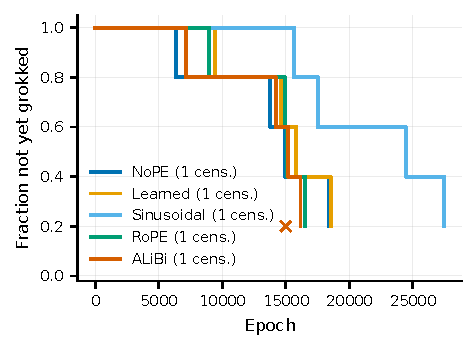
\includegraphics[width=\columnwidth]{figures/fig2_onset_survival.pdf}
\caption{Fraction of runs not yet grokked vs.\ epoch, per PE (core grid,
$n{=}5$ seeds each; $\times$ marks censoring). Sinusoidal (light blue) is the
outlier: no run groks by the 15k horizon; extensions resolve all its onsets at
15.6k--27.5k.}
\label{fig:survival}
\end{figure}

\begin{figure}[t]
\centering
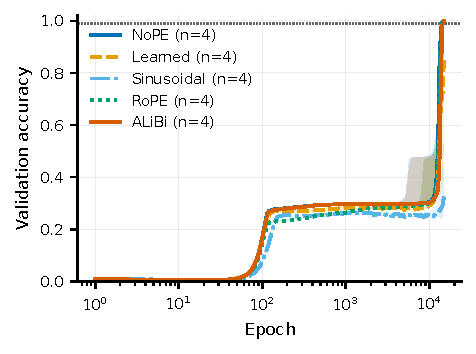
\includegraphics[width=\columnwidth]{figures/fig1_dynamics.pdf}
\caption{Validation accuracy (median with IQR band across seeds) per PE.
All conditions share the memorization plateau at 25--30\%; PE shifts the
timing of the transition.}
\label{fig:dynamics}
\end{figure}

\section{H2: Circuits Converge Across PEs}

\paragraph{All grokked runs learn the same algorithm.} Every grokked run,
under every PE, ends with restricted loss $\approx 0$ (the top-5 Fourier
frequencies alone solve the task), excluded loss 11.5--17.9 (removing them
destroys training performance), and embedding Fourier concentration
0.83--0.88---the delayed sinusoidal runs included, whose final concentration
(0.88) is the highest of all conditions (Figure~\ref{fig:signatures}). At the
algorithmic level this extends circuit-universality claims
\cite{mccracken2025universal,moisescu2025unifying} along the PE axis.

\paragraph{But PE selects the implementation's attention-dependence.} The
pre-registered label-permutation test on matched post-grok signature vectors
(all runs $\ge$1{,}000 epochs past onset, balanced $n{=}20$, 4 per PE) is
strongly positive: $\eta^2{=}0.37$, $p{=}0.001$. The separation is carried by
the attention-facing metrics, not the Fourier metrics: uniform-attention
ablation $\Delta$loss groups the PEs by \emph{where they inject position} ---
attention-level PEs yield circuits nearly indifferent to attention ablation
(RoPE 1.19, ALiBi 1.96 median $\Delta$), while embedding-level or absent PEs
yield strongly attention-dependent circuits (NoPE 4.00, sinusoidal 4.19,
learned 5.59). Interpretation (post hoc): when positional structure is
supplied inside the attention computation, the model can implement the
Fourier mixing in a position-agnostic way; when it is not, the learned
attention pattern itself becomes a load-bearing part of the circuit.

\paragraph{Trajectories tie circuit formation to grokking.} Embedding
Fourier concentration rises at each run's grokking onset (within one
checkpoint in all resolved-onset runs) and never rises in runs that have not
grokked (Figure~\ref{fig:trajectories}): circuit formation and generalization
are one event whose \emph{timing} PE controls.

\begin{figure}[t]
\centering
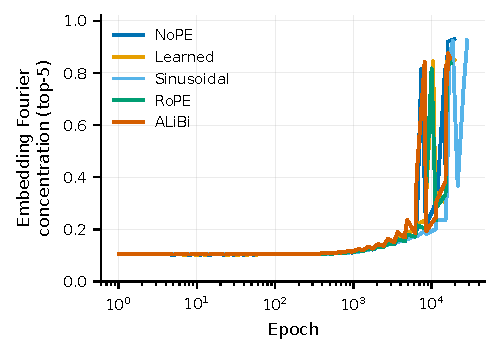
\includegraphics[width=\columnwidth]{figures/fig3_signature_trajectories.pdf}
\caption{Median embedding Fourier concentration vs.\ epoch, per PE. The rise
coincides with grokking onset; sinusoidal's concentration stalls near 0.33
through the 15k horizon (its extensions complete the same rise later).}
\label{fig:trajectories}
\end{figure}

\begin{figure}[t]
\centering
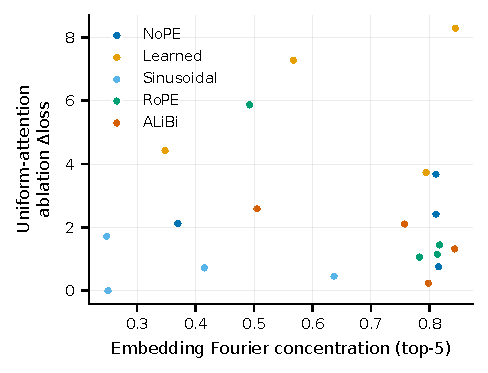
\includegraphics[width=\columnwidth]{figures/fig4_final_signatures.pdf}
\caption{Final circuit signatures (embedding Fourier concentration vs.\
uniform-attention ablation $\Delta$loss), colored by PE. Grokked runs cluster
at high concentration regardless of PE.}
\label{fig:signatures}
\end{figure}

\begin{table}[t]
\centering
\small
\begin{tabular}{lrrrrr}
\toprule
 & NoPE & Learn. & Sinus. & RoPE & ALiBi \\
\midrule
Grokked (15k) & 3/5 & 2/5 & 0/5 & 3/5 & 3/5 \\
Median onset & 14.4k & 15.2k & 21.0k & 15.0k & 14.7k \\
Fourier conc. & 0.87 & 0.84 & 0.88 & 0.83 & 0.85 \\
Restr.\ loss & 0.00 & 0.00 & 0.00 & 0.00 & 0.00 \\
Unif.-abl.\ $\Delta$ & 4.00 & 5.59 & 4.19 & 1.19 & 1.96 \\
\bottomrule
\end{tabular}
\caption{Per-PE summary (core condition; onsets include 40k extensions;
signature medians over grokked runs). Full per-run table in the repository.}
\label{tab:summary}
\end{table}

\section{H3: Signatures, Not PE Labels, Predict OOD}

On the OOD grid (operand rows $a \in [100,112]$ excluded from all training
data), grokked runs transfer almost perfectly to the held-out rows
(99.6--99.9\% accuracy) while non-grokked runs sit at 16--27\%. Because most
PE conditions contain both outcomes across seeds, the PE label is uninformative
about OOD accuracy (leave-one-out $R^2{=}-1.59$), while the six-metric circuit
signature predicts it almost perfectly ($R^2{=}0.92$; Spearman
$\rho{=}0.94$; $n{=}10$, modest-$n$ supporting evidence as pre-registered).
Figure~\ref{fig:ood} shows OOD accuracy against final Fourier concentration.

\begin{figure}[t]
\centering
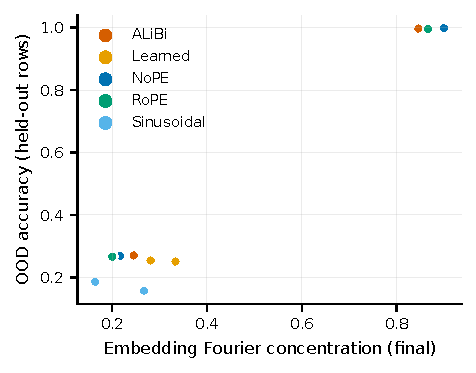
\includegraphics[width=\columnwidth]{figures/fig5_ood_vs_signature.pdf}
\caption{OOD accuracy on held-out operand rows vs.\ final embedding Fourier
concentration, colored by PE. The signature separates the outcomes; the PE
label does not.}
\label{fig:ood}
\end{figure}

\section{Discussion}

\paragraph{Why would sinusoidal APE interfere?} The grokked circuit stores
task frequencies in the token-embedding spectrum. Sinusoidal APE injects
fixed, dense sinusoids of unrelated frequencies into that same subspace at
every step; unlike learned APE (which can adapt) or RoPE/ALiBi (which act on
attention, not the embedding), it cannot get out of the way. The signature
trajectories are consistent with interference-then-recovery: sinusoidal runs'
concentration stalls near 0.33 for tens of thousands of epochs, then completes
the standard transition. We offer this as a hypothesis; testing it (e.g., by
orthogonalizing the PE against task frequencies) is future work.

\paragraph{Same algorithm, different timing and location.} Combined, H1--H3
support a two-level picture: PE choice leaves the learned \emph{algorithm}
invariant (Fourier multiplication, in every condition) while controlling its
\emph{schedule} (when it forms; sinusoidal latest) and its \emph{location}
(inside learned attention patterns for embedding-level/absent PEs; outside
them for attention-level PEs). Practically: PE ablations in small-model
interpretability studies change time-to-solution and ablation-robustness, not
solution identity; horizon-limited PE comparisons can silently misclassify
slow conditions as failures; and uniform-attention ablations---a standard
circuit probe---measure a PE-dependent property, not an
architecture-independent one.

\paragraph{Limitations.} Single task family ($p{=}113$ addition; other moduli
and operations were pre-planned but cut for compute budget), single
architecture scale (0.23M parameters, 1 layer), 4--5 seeds per condition,
CPU-only horizon of 15k/40k epochs, and an OOD design limited to operand-row
holdout with $n{=}10$. Rank tests across PEs are underpowered at this seed
count: the sinusoidal horizon effect and the signature separation are the only
claims exceeding the measured noise floor, and the attention-dependence
grouping, while significant under the pre-registered test, has a post-hoc
interpretation. Circuit signatures are logit- and embedding-level; we do not
analyze neuron-level implementations.

\section{Reproducibility}

All code, seeds, per-epoch CSV logs, and analysis/figure pipelines are
released; datasets are synthesized deterministically ($p$, operation,
fraction, seed). Every number and figure regenerates via two commands
(\texttt{analysis --all}; \texttt{figures --all}); the headline matched
post-grok test is the committed \texttt{analysis --matched} path, which
reproduces $\eta^2{=}0.368$, $p{=}0.001$, $n{=}20$ from the released logs.
Training is bit-exact resumable and device-agnostic; the full 50-run grid
used $\sim$22 h on one 8-core consumer CPU (no GPU). The reproducibility
checklist follows the references.

\section*{AI-Use Statement}

In accordance with AAAI policy on AI systems in publications: this project's
experiments, code, analysis, and manuscript drafting were performed with
substantial assistance from an AI system (an LLM-based research agent),
directed and reviewed by the human author, who takes full responsibility for
all content. The AI system is not an author and is not cited as a source; all
citations were verified against their original sources by direct retrieval.
Experimental decisions are documented in a public decision log in the released
repository.

\bibliography{references}

\end{document}
